\documentclass[12pt]{article}

\usepackage[margin=0.8in, landscape]{geometry}
\usepackage{fancyhdr}
\usepackage{hyperref}
\usepackage{xcolor}
\usepackage{tikz}
\usepackage{enumitem}
\usepackage{array}
\usepackage{longtable}
\usetikzlibrary{arrows.meta, positioning, shapes.geometric, fit, backgrounds}

\hypersetup{
    colorlinks=true,
    linkcolor=blue,
    urlcolor=blue
}

\pagestyle{fancy}
\fancyhf{}
\lhead{Workflow Diagram}
\rhead{Product Expiration Tracking App}
\cfoot{\thepage}

\title{High-Level Workflow Diagram\\Product Expiration Tracking Application}
\author{Prepared for Course Project}
\date{\today}

\definecolor{uiBlue}{RGB}{219,235,255}
\definecolor{apiGreen}{RGB}{223,246,221}
\definecolor{dataYellow}{RGB}{255,246,214}
\definecolor{securityPink}{RGB}{255,229,229}
\definecolor{notifyPurple}{RGB}{239,229,255}
\definecolor{infraGray}{RGB}{240,240,240}

\begin{document}

\maketitle
\thispagestyle{fancy}

\section*{Purpose}
This document provides a high-level workflow diagram for the Product Expiration Tracking Application. The diagram explains how a user connects to the mobile user interface, how the frontend communicates with the backend, where the user's data is stored, and which parts of the system can access that data. The current project scope supports manual product entry only.

\section*{High-Level System Workflow}



\begin{center}
\resizebox{0.96\textwidth}{!}{%
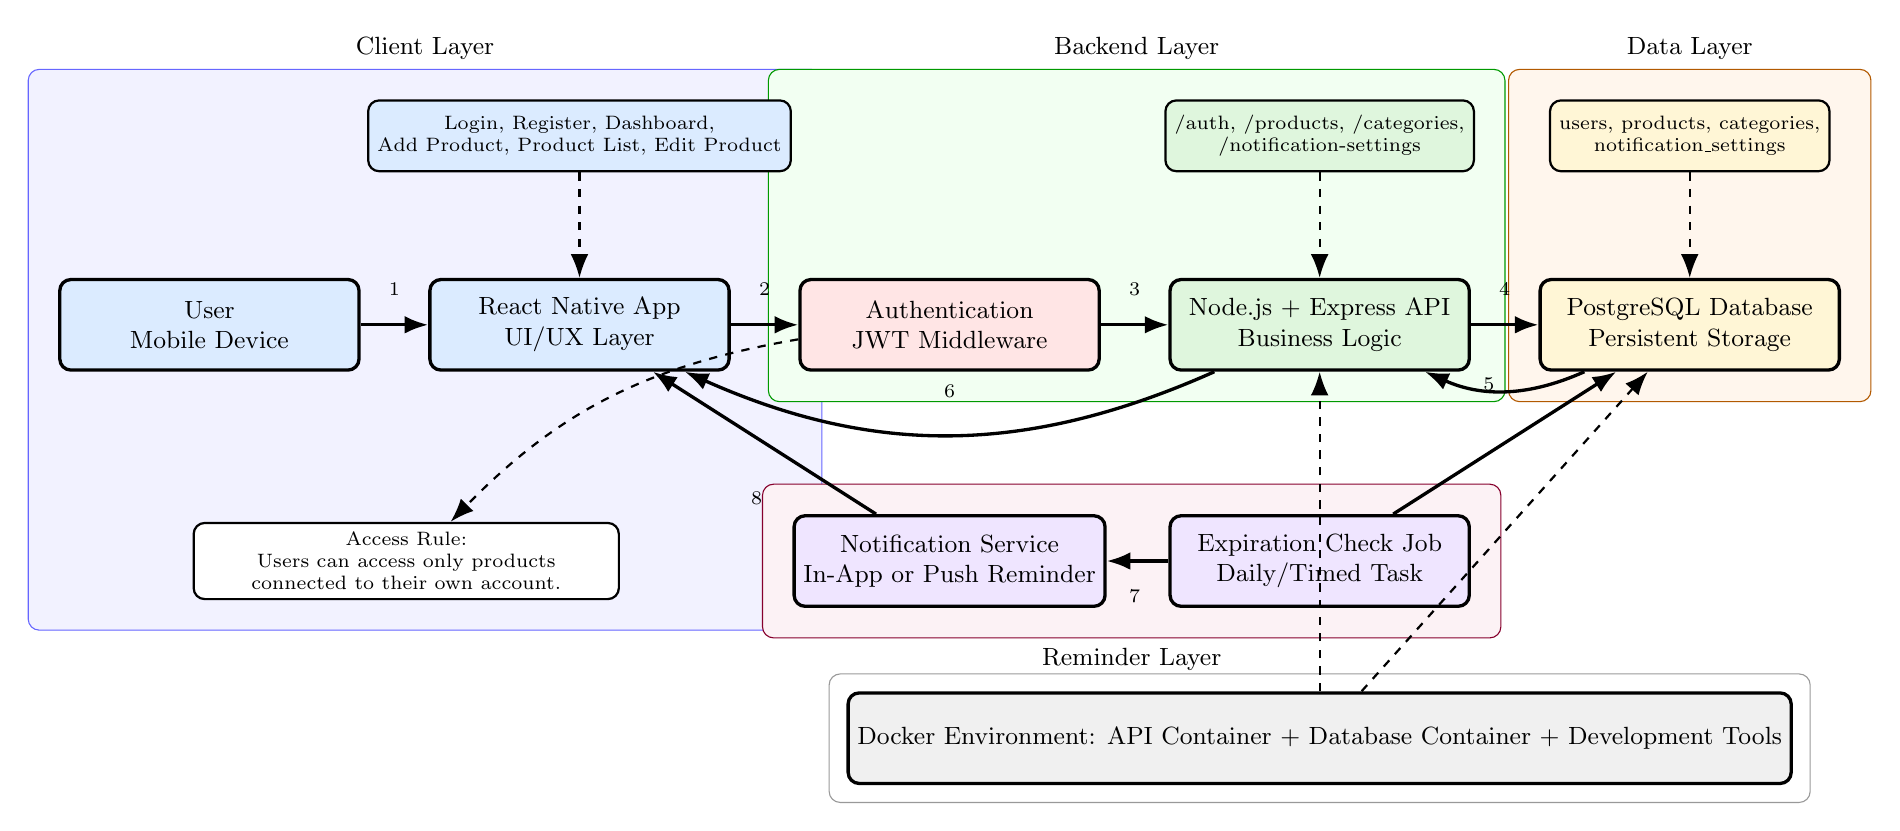
\begin{tikzpicture}[
    box/.style={rectangle, rounded corners, draw=black, very thick, align=center, minimum width=3.8cm, minimum height=1.15cm, font=\small},
    smallbox/.style={rectangle, rounded corners, draw=black, thick, align=center, minimum width=3.35cm, minimum height=0.9cm, font=\scriptsize},
    arrow/.style={-{Latex[length=3mm]}, very thick},
    dashedarrow/.style={-{Latex[length=3mm]}, thick, dashed}
]

% Main data flow
\node[box, fill=uiBlue] (user) at (0,0) {User\\Mobile Device};
\node[box, fill=uiBlue] (app) at (4.7,0) {React Native App\\UI/UX Layer};
\node[box, fill=securityPink] (auth) at (9.4,0) {Authentication\\JWT Middleware};
\node[box, fill=apiGreen] (api) at (14.1,0) {Node.js + Express API\\Business Logic};
\node[box, fill=dataYellow] (db) at (18.8,0) {PostgreSQL Database\\Persistent Storage};

% Supporting components
\node[smallbox, fill=uiBlue] (screens) at (4.7,2.4) {Login, Register, Dashboard,\\Add Product, Product List, Edit Product};
\node[smallbox, fill=apiGreen] (routes) at (14.1,2.4) {/auth, /products, /categories,\\/notification-settings};
\node[smallbox, fill=dataYellow] (tables) at (18.8,2.4) {users, products, categories,\\notification\_settings};
\node[box, fill=notifyPurple] (notif) at (9.4,-3.0) {Notification Service\\In-App or Push Reminder};
\node[box, fill=notifyPurple] (scheduler) at (14.1,-3.0) {Expiration Check Job\\Daily/Timed Task};
\node[box, fill=infraGray, minimum width=9.5cm] (docker) at (14.1,-5.25) {Docker Environment: API Container + Database Container + Development Tools};
\node[smallbox, fill=white, minimum width=5.4cm] (privacy) at (2.5,-3.0) {Access Rule:\\Users can access only products\\connected to their own account.};

% Main arrows, numbered in explanation below
\draw[arrow] (user) -- (app);
\draw[arrow] (app) -- (auth);
\draw[arrow] (auth) -- (api);
\draw[arrow] (api) -- (db);
\draw[arrow] (db) to[bend left=24] (api);
\draw[arrow] (api) to[bend left=24] (app);

% Supporting arrows
\draw[dashedarrow] (screens) -- (app);
\draw[dashedarrow] (routes) -- (api);
\draw[dashedarrow] (tables) -- (db);
\draw[arrow] (scheduler) -- (db);
\draw[arrow] (scheduler) -- (notif);
\draw[arrow] (notif) -- (app);
\draw[dashedarrow] (auth) to[bend right=18] (privacy);
\draw[dashedarrow] (docker) -- (api);
\draw[dashedarrow] (docker) -- (db);

% Step labels
\node[font=\scriptsize] at (2.35,0.45) {1};
\node[font=\scriptsize] at (7.05,0.45) {2};
\node[font=\scriptsize] at (11.75,0.45) {3};
\node[font=\scriptsize] at (16.45,0.45) {4};
\node[font=\scriptsize] at (16.25,-0.75) {5};
\node[font=\scriptsize] at (9.4,-0.85) {6};
\node[font=\scriptsize] at (11.75,-3.45) {7};
\node[font=\scriptsize] at (6.95,-2.2) {8};

% Background groups
\begin{pgfonlayer}{background}
\node[draw=blue!60, fill=blue!5, rounded corners, fit=(user)(app)(screens)(privacy), inner sep=0.38cm, label={[font=\small]above:Client Layer}] {};
\node[draw=green!60!black, fill=green!5, rounded corners, fit=(auth)(api)(routes), inner sep=0.38cm, label={[font=\small]above:Backend Layer}] {};
\node[draw=orange!70!black, fill=orange!7, rounded corners, fit=(db)(tables), inner sep=0.38cm, label={[font=\small]above:Data Layer}] {};
\node[draw=purple!70!black, fill=purple!5, rounded corners, fit=(scheduler)(notif), inner sep=0.38cm, label={[font=\small]below:Reminder Layer}] {};
\node[draw=gray!80, rounded corners, fit=(docker), inner sep=0.22cm] {};
\end{pgfonlayer}

\end{tikzpicture}%
}
\end{center}

\vspace{0.3cm}
\noindent\textbf{Diagram step key:} 1) User opens the app. 2) App sends a protected request. 3) Backend verifies authentication. 4) API reads or writes product data. 5) Database returns data. 6) API returns JSON to the mobile app. 7) Expiration job creates reminders. 8) Reminder is shown to the user.

\newpage

\section*{Workflow Explanation}

\begin{enumerate}[leftmargin=*]
    \item \textbf{User opens the mobile app.} The user interacts with the React Native mobile application from a phone or tablet.
    \item \textbf{User signs in or creates an account.} The app sends login or registration information to the Node.js backend. After successful login, the backend returns a JSON Web Token (JWT).
    \item \textbf{User manually enters product information.} The user types product name, category, quantity, storage location, purchase date, expiration date, and optional notes.
    \item \textbf{Frontend sends requests to the backend.} The React Native app sends HTTPS requests to the Node.js and Express API. Protected requests include the user's JWT token.
    \item \textbf{Backend validates and processes data.} The backend checks the request, verifies the authenticated user, validates product fields, and applies business rules.
    \item \textbf{Data is stored in the database.} Product data is saved in PostgreSQL. Each product record is connected to the correct user account so users can access only their own data.
    \item \textbf{Products are displayed back to the user.} The backend returns JSON responses to the mobile app, and the React Native interface displays product lists, expiration status, and product details.
    \item \textbf{Expiration reminders are generated.} A scheduled backend job checks stored expiration dates and creates reminders for products that are near expiration or already expired.
\end{enumerate}

\section*{Data Access Overview}

\begin{longtable}{|p{0.22\linewidth}|p{0.34\linewidth}|p{0.34\linewidth}|}
\hline
\textbf{System Part} & \textbf{What It Can Access} & \textbf{Purpose} \\
\hline
React Native Mobile App & User-entered product data returned by the API for the logged-in user only & Displays screens, forms, product lists, and reminders \\
\hline
Node.js/Express API & User accounts, product records, categories, and notification settings & Validates requests, applies business rules, and controls access to data \\
\hline
PostgreSQL Database & Stored users, products, categories, and reminder settings & Provides persistent storage for application data \\
\hline
Authentication Middleware & Login credentials during sign-in and JWT tokens during protected requests & Confirms that only authenticated users can access private product data \\
\hline
Scheduled Expiration Job & Product names, expiration dates, and reminder settings & Finds products close to expiration and triggers reminders \\
\hline
Administrator/Developer & System logs and deployment tools; no direct use of personal product data is required for normal support & Maintains deployment, fixes bugs, and monitors system health \\
\hline
\end{longtable}

\section*{Security and Privacy Notes}

\begin{itemize}[leftmargin=*]
    \item Users must be authenticated before they can create, view, update, or delete product records.
    \item Each product belongs to one user account, and backend authorization rules prevent one user from accessing another user's products.
    \item Passwords should be stored using a secure hashing library such as bcrypt.
    \item API communication should use HTTPS in production.
    \item Environment variables should store secrets such as database passwords, JWT secrets, and service configuration.
    \item The current version does not use barcode scanning, image scanning, or artificial intelligence scanning.
\end{itemize}

\section*{Docker Deployment Overview}

The project can be organized into a multi-container Docker environment. A typical development deployment may include the following services:

\begin{longtable}{|p{0.24\linewidth}|p{0.30\linewidth}|p{0.36\linewidth}|}
\hline
\textbf{Container/Service} & \textbf{Main Technology} & \textbf{Responsibility} \\
\hline
Mobile Build/Frontend Service & React Native, Node package manager, Expo or React Native CLI & Builds and runs the mobile frontend during development \\
\hline
Backend API Service & Node.js, Express.js & Handles authentication, product APIs, validation, and reminder logic \\
\hline
Database Service & PostgreSQL & Stores users, manually entered products, categories, and reminder settings \\
\hline
Optional Admin Tool & pgAdmin or database client & Helps developers inspect database tables during development \\
\hline
\end{longtable}

\section*{Summary}

At a high level, the user connects through the React Native mobile interface. The mobile app sends authorized requests to a Node.js and Express backend. The backend validates user actions, protects access with authentication, and stores product expiration information in PostgreSQL. A scheduled backend process checks expiration dates and sends reminders back to the user interface. The complete system can be packaged using Docker containers for easier development and deployment.

\end{document}
